\documentclass[9pt]{article}

\usepackage{amsmath}
\usepackage{tcolorbox}
% `parskip` removes indentation for all paragraphs: http://tex.stackexchange.com/a/55016
\usepackage{parskip}
% Allows us to color rows / cols of a table.
% See https://texblog.org/2011/04/19/highlight-table-rowscolumns-with-color/
\usepackage{color, colortbl}

\usepackage{hyperref}
\graphicspath{{images/ps2b/}}

\leftmargin=0.25in
\oddsidemargin=0.25in
\textwidth=6.0in
\topmargin=-0.25in
\textheight=9.25in

\definecolor{Gray}{gray}{0.9}

\begin{document}

\begin{center}
  \large\textbf{MIT 18.01 Problem Set 2B Unofficial Solutions}
\end{center}

\begin{tcolorbox}
  \renewcommand{\thefootnote}{\roman{footnote}}
  \textbf{Q1) Golf balls} The area of a section of a sphere of radius $R$ between two parallel planes that are a distance $h$ apart is \footnote{This formula will be derived in Unit 4. Two examples may convince you that it is reasonable. For $h = R$, it gives the area of the hemisphere, $2 \pi R^2.$ For $h = 2R$ it gives $4 \pi R^2$, the area of the whole sphere.}\\
  \begin{center}
    area of a spherical section = $2 \pi h R$
  \end{center}
  \ \\
  Slice the sphere of radius $R$ by a horizontal plane. The portion of the plane inside the sphere is a disk of radius $r \leq R$. The portion of the spherical surface above the plane is called a \emph{spherical cap}. For example, if the plane passes through the center, then the disk has radius $r = R$, its circumference is the equator, and the spherical cap is the Northern Hemisphere. More generally, a spherical cap is the portion of surface of the Earth north of a latitude line. The formula above applies to regions between two latitude lines, and, in particular, to spherical caps.\\
  \\
  a) Consider a spherical cap which is the portion of the surface of the sphere above horizontal plane that slices the sphere at or above its center. Find the area of the cap as a function of $R$ and $r$. Do this by finding first the formula for the height $h$ of the spherical cap in terms of $r$ and $R$. (This height is the vertical distance from the horizontal slicing plane to the North Pole.) Then use your formula for $h$ and the formula above for the area of spherical sections.
\end{tcolorbox}

\begin{center}
  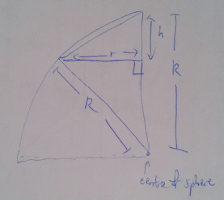
\includegraphics[scale=0.8]{q1a.jpg}
\end{center}

In the above diagram, we see that the distance between the 2 horizontal slicing planes is $R - h$, where $h$ is the height of the spherical cap. The insight is that, the distance from the center of the sphere to any point on the circumference is $R$. We form a right triangle using this line and the line with the radius $r$ of the spherical cap.

By the Pythagorean formula, $(R - h)^2 = R^2 - r^2$. Hence

\begin{align*}
  R - h &= \sqrt{R^2 - r^2}\\
  h &= R - \sqrt{R^2 - r^2}
\end{align*}

Then the area of the spherical cap is $2 \pi h R = 2 \pi (R - \sqrt{R^2 - r^2}) R = 2 \pi R (R - \sqrt{R^2 - r^2})$


\begin{tcolorbox}
  \textbf{Q1b)} Express the formula for the area of a spherical cap in terms of $R^2$ and $r / R$. (This is natural because the proportional scaling $cr$ and $cR$ changes the area by the factor $c^2$.) Then use the linear and quadratic approximations to $(1 + x)^{1/2}$ near $x = 0$ to find a good and an even better approximation to the area of the spherical cap, appropriate when the ratio $r / R$ is small. (Hint: What is $x$?) Simplify your answers as far as possible: the approximation corresponding to the linear approximation to $(1 + x)^{1/2}$ should be very familiar.
\end{tcolorbox}

In part (a), we see that the area of the spherical cap is $2 \pi R (R - \sqrt{R^2 - r^2})$. This can also be expressed as

\begin{align*}
  2 \pi R (R - \sqrt{R^2 - r^2}) &= 2 \pi R (R - \sqrt{R^2 (1 - \frac{r^2}{R^2})}) \\
                                 &= 2 \pi R (R - R \sqrt{1 - \frac{r^2}{R^2}}) \\
                                 &= 2 \pi R^2 (1 - \sqrt{1 - \frac{r^2}{R^2}}) \\
\end{align*}

When $\frac{r}{R}$ is small, $\frac{r^2}{R^2} \approx 0$. Let $x = -\frac{r^2}{R^2}$. We are going to use the linear approximation of $(1 + x)^{1/2}$. Let $f(x) = (1 + x)^{1/2}$. Then $f(0) = (1 + 0)^{1/2} = 1$ and $f'(x) = \frac{1}{2} (1 + x)^{-1/2}$ and $f'(0) = \frac{1}{2}(1 + 0)^{-1/2} = \frac{1}{2}$.

Hence the linear approximation to $(1 + x)^{1/2} = f(0) + f'(0)(x - 0) = 1 + \frac{1}{2}x$ and the linear approximation to $\sqrt{1 - \frac{r^2}{R^2}}$ is thus $1 + \frac{1}{2}(-\frac{r^2}{R^2}) = 1 - \frac{r^2}{2R^2}$

Linear approximation to area of spherical cap is thus $2 \pi R^2 (1 - (1 - \frac{r^2}{2R^2})) = 2 \pi R^2 (\frac{r^2}{2R^2}) = \pi r^2$

For quadratic approximation to $\sqrt{1 - \frac{r^2}{R^2}}$, we need to compute the 2nd derivative of $f(x) = (1 + x)^{1/2}$, which is $f''(x) = -\frac{1}{4}(1 + x)^{-3/2}$. Now, $f''(0) = -\frac{1}{4}(1 + 0)^{-3/2} = -\frac{1}{4}$

Hence, quadratic approximation to $\sqrt{1 - \frac{r^2}{R^2}}$ is:

\begin{align*}
  1 + \frac{1}{2}(-\frac{r^2}{R^2} - 0) - \frac{\frac{1}{4}}{2}(-\frac{r^2}{R^2} - 0)^2 &= 1 - \frac{r^2}{2R^2} - \frac{r^4}{8R^4}
\end{align*}

Quadratic approximation to area of spherical cap is

\begin{align*}
  2 \pi R^2 (1 - (1 - \frac{r^2}{2R^2} - \frac{r^4}{8R^4})) &= 2 \pi R^2 (\frac{r^2}{2R^2} + \frac{r^4}{8R^4}) \\
                                                            &= \pi r^2 + \pi \frac{r^4}{4R^2}
\end{align*}


\begin{tcolorbox}
  \textbf{Q1c)} The following problem appeared on a middle school math contest exam. The numbers have been changed to protect the innocent. Consider a golf ball that is 3 centimeters in diameter with 100 hemispherical dimples of diameter 3 millimeters. (Note that this is not a realistic golf ball because the dimples are too deep). Find the area of the golf ball rounded to the nearest $1/100$ of a square centimeter using the approximation $\pi \approx 3.14$. (The students were given three minutes. We are spending more time on it.) \\

  Under the rules of the contest, an incorrectly rounded answer was counted as wrong with no partial credit, so correct numerical approximations were crucial. Some students objected that they could not figure out the area of portion of the large sphere that is removed when a dimple is inserted. A careless examiner had assumed that the students would use the approximation that the area removed for each dimple was nearly the same as the area of a flat disk. We are going to figure out whether this approximation is adequate or gives the wrong answer according to the rules.\\

  Write down formulas for the surface area of the golf ball in the three cases listed below. (Put in 100 dimples, but leave $r, R$, and $\pi$ as letters.)\\
  \\
  i) the approximation pretending that the removed surface is flat (what is the relationship between this and the approximations of part (b)?)\\
  \\
  ii) the higher order approximation you derived in part (b)\\
  \\
  iii) the exact formula\\

  Finally, evaluate each of the answers for the given values $r = .15$ and $R = 1.5$ centimeters, and find the accuracy of the approximations.
\end{tcolorbox}


\begin{tcolorbox}
  \textbf{Q1d)} Although nobody noticed it at the time, the examiner who created this problem made a much bigger mistake. With the diameters actually given, it would have been impossible for the number of dimples given to be placed on the golf ball without overlap. Give a (reasonable) estimate for the largest number of dimples that can fit on our golf ball.
\end{tcolorbox}


\begin{tcolorbox}
  \textbf{Q2)} Draw the graph of $f(x) = 1/(1 + x^2)$ and, directly underneath, it with the graphs of $f'(x)$ and $f''(x)$. Label critical points and inflection points on the graph of $f$ with their coordinates. Draw vertical lines joining these special points of the graph of $f$ to the corresponding points on the graphs below.
\end{tcolorbox}

\end{document}
